\documentclass{beamer}

\usepackage{siunitx}
\usepackage{graphicx}

\usetheme{Montpellier}

\title{Effect of low-rise building geometry on tornado-induced loads}
\author{140926~WANG Yong}
\institute{Southeast University}
\date{\today}

\begin{document}

\begin{frame}
	\titlepage
\end{frame}

\section*{Outline}
\begin{frame}
	\tableofcontents
\end{frame}

\section{Introduction}

\begin{frame}
    \frametitle{Challenges to quantify  tornado-induced loads:}
    \begin{itemize}
    	\item<1-> Lack of research facilities capable of determining tornado-induced loads (pressures, forces, etc.)
    	\item<2-> Absence of full-scale data
    	\item<3-> Lack of interest in tornado-resistant design
    \end{itemize}
\end{frame}

\begin{frame}
    \frametitle{How to overcome these challenge:}
    \begin{itemize}
    	\item<1-> Iowa State University (ISU) tornado simulator
    	\item<2-> Full-scale data from several recent tornados
    	\item<3-> Pressures obtained form  the ISU simulator are verified
    \end{itemize}
\end{frame}


\section{Description of simulated tornado}
\subsection{Maximum horizonal wind speed}

\begin{frame}
	\frametitle{Maximum horizontal wind speed}
	\begin{description}
		\item[Fact 1:  ]<1-> Around 90\% of all tornados are rated F2 or less
		\item[Fact 2: ]<2-> Maximum velocity of F2 tornado is \alert{\SI{74}{m/s}}
		\item[Fact 3: ]<3-> Design wind speed ranges from \alert{\SI{63}{m/s}} to \alert{\SI{80}{m/s}} (ASCE 7-10, 2010)
		\item[Fact 4: ]<4-> Maximum horizonal velocity of the tornado generated by ISU Simulator is \alert{\SI{11.7}{m/s}}
	\end{description}
	\begin{block}<5->{Choose target full-scale wind speed to be \alert{\SI{74}{m/s}}}
			 Velocity scale $\lambda_v=11.7/74=1/6.3$
	\end{block} 
\end{frame}

\begin{frame}
	\frametitle{Contour plot of normalized tangential velocity}
	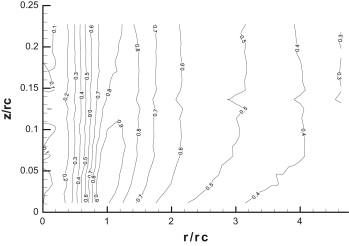
\includegraphics{./fig/1.jpg}
\end{frame}

\subsection{Tornado vortex diameter}

\begin{frame}
	\frametitle{Tornado vortex diameter}
	\begin{definition}
	 	\alert{Radius of the core $r_c$}: radius of the maximum wind near the ground
	\end{definition}
	\begin{description}
		\item[Fact 1: ]<2-> $r_c$ of F2 tornado is between \alert{\SI{45}{} to \SI{225}{m}}
		\item[Fact 2: ]<3-> $r_c$ of simulated tornado is \alert{\SI{0.56}{m}}
	\end{description}
	\begin{block}<4->{Choose $r_c$ of target full-scale tornado to be \alert{\SI{56}{m}}}
		   Length scale is $1:100$ 
	\end{block} 

\end{frame}

\subsection{Swirl ratio}

\begin{frame}
	\frametitle{Swirl ratio: definition}
	\begin{definition}
		\alert{Swirl ratio $S$}: 
		$$ S = \frac{\pi V_{\theta\mathrm{max}} r_c^2}{Q}$$
		\begin{description}
			\item[$r_c$: ] core radius
			\item[$V_{\theta\mathrm{max}}$: ] maximum tangential wind speed
			\item[$Q$: ] inflow rate of the vortex measured at $r=r_c$
		\end{description}
	\end{definition}
\end{frame}

\begin{frame}
	\frametitle{How to choose swirl ratio}
		\begin{description}
			\item[Fact 1: ] <2-> Data from full-scale tornados indicates \alert{$S\geqslant2.0$}
			\item[Fact 2: ]<3-> Best fit of full-scale data with numerical simulation when \alert{$S\geqslant2.0$}
		\end{description}
		\begin{block}<4->{Choose the swirl ratio $S$  to be \alert{\num{2.6}} }
			
		\end{block}
\end{frame}


\section{Model description, instruments,  conventions}
\subsection{Building models}
\subsection{Instrumentation}
\subsection{Procedure and conventions}

\section{Results}
\subsection{The effect of cave height}
\subsection{The effect of roof pitch}
\subsection{The effect of the ratio plan dimension}

\section{Conclusions}


\begin{frame}
\end{frame}



\end{document}